\section{Navigation in Disp3D}

This section describes how to navigate through the 3D control widget of the Disp3D example.

\begin{aims}
	\item[\hspace*{10mm} Where to Navigate] The two new items that use the new features can be found under\\ \textit{sample/Right visual/MEG Data} \ding[1.4]{182} and \textit{sample/Right visual/EEG Data}. \ding[1.4]{183} \\ 
	MEG data utilizes the Sensor Surface under \textit{Sensors/VectorView/Sensor Surface} \ding[1.4]{182}, while EEG data uses the Head surface under \textit{sample/BEM/Head}. \ding[1.4]{183} 
\end{aims}
	
	
\begin{aims}
	\item[\hspace*{10mm} Turning Data Streams On/Off] Click the checkbox "Stream data on/off" to toggle data streaming. All necessary calculations are executed and the interpolation begins. \ding[1.4]{184}
\end{aims}

\begin{aims}
	\item[\hspace*{10mm} Choosing a Color Map] Click on the second row of text and then choose an entry of the droplist to switch color maps. \ding[1.4]{185}
\end{aims}

\begin{aims}
	\item[\hspace*{10mm} Configuring Normalization Thresholds] Click on the third row of text and then click left inside the arising graph for the lower threshold and right for the upper threshold. 
	Unwanted activation can be hidden this way. \ding[1.4]{186}
\end{aims}

\begin{aims}
	\item[\hspace*{10mm} Editing sample delays] Use the spinbox in the fourth row to decrease / increase the delay between visual outputs. \ding[1.4]{187}
\end{aims}

\begin{aims}
	\item[\hspace*{10mm} Toggling Data Looping] Click the checkbox in the fifth row to toggle looping of the last received block of sensor data. \ding[1.4]{188}
\end{aims}

\begin{aims}
	\item[\hspace*{10mm} Sample Averaging] Use the spinbox in the sixth row to decrease / increase the number of samples that should be averaged to one signal. \ding[1.4]{189}
\end{aims}

\begin{aims}
	\item[\hspace*{10mm} Distance Threshold] Use the spinbox in the seventh row to decrease / increase the distance threshold that is used when running the SCDC and the creation of the interpolation matrix. By doing this less / more vertices around the sensor locations are considered during  the interpolation. \ding[1.4]{190}
\end{aims}

\begin{aims}
	\item[\hspace*{10mm} Interpolation Function] Use the droplist in the last row to choose a function to use during the creation of the interpolation matrix. \ding[1.4]{191}
\end{aims}


\begin{center}
		\hspace{-1.4cm}
		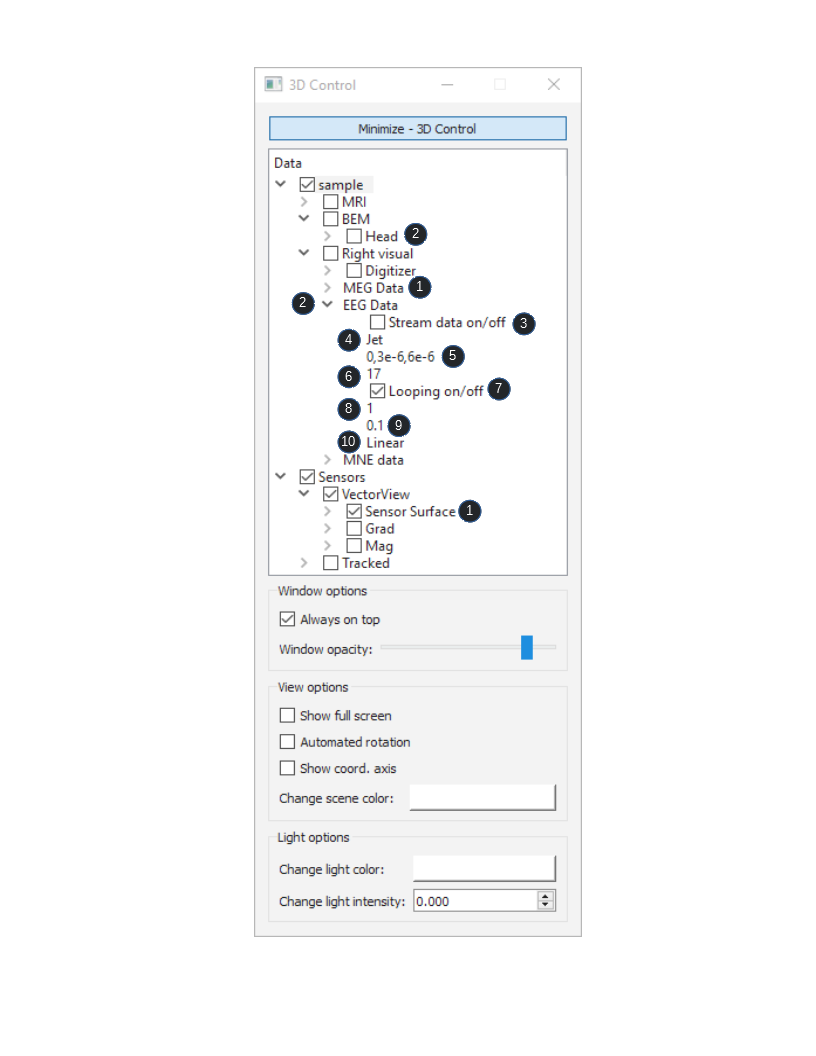
\includegraphics[scale=0.8]{figures/disp3D.png}
	
\end{center}


